\title{\color{ladrillo}\bfseries De los Jueces a David\\[4pt]\large\color{cafe}\mdseries Un pueblo que quiso ser como las naciones y un remanente que esperó al rey según el corazón de Dios}
\author{}\date{\color{sepia}Serie «Israel, el pueblo de Dios» · Estudio 3}
\begin{document}
\maketitle\thispagestyle{empty}

\begin{abstract}\noindent
Este tercer estudio recorre la historia de Israel desde la muerte de Josué hasta la unción de David y muestra que, en la etapa más oscura de su vida en la tierra, Dios no desampara a su pueblo y siembra las promesas de restauración que retomarán los profetas y que Pablo invocará en Romanos 11. El pueblo llamado a ser «reino de sacerdotes y nación santa» (Éx 19:6) se corrompe desde dentro hasta repetir en Guibeá el pecado de Sodoma y acaba pidiendo un rey «como todas las naciones» (1~S 8:5). En medio de esa ruina Dios levanta libertadores, preserva un remanente, incorpora a una moabita al linaje de David y anuncia por boca de Ana un rey «ungido» (\emph{mashíaj}, 1~S 2:10). La promesa de que «YHWH no desamparará a su pueblo» (1~S 12:22) reaparece en Isaías, Jeremías y Oseas como esperanza de jueces restaurados, de un renuevo de Isaí y de un regreso a «David su rey», y Pablo la recoge casi a la letra en Ro 11:1--2.
\par\smallskip\noindent\textbf{Palabras clave:} Jueces, Rut, Samuel, Saúl, David, ungido, remanente, Isaías, Jeremías, Romanos 11.
\end{abstract}

\section{Introducción}

¿Qué ocurre cuando el pueblo de Dios se cansa de ser distinto? Jueces, Rut y 1~Samuel responden con una historia de casi dos siglos en la que Israel, ya instalado en la tierra, sirve a los baales de sus vecinos y termina pidiendo un rey «como todas las naciones» (1~S 8:5). La vocación no se pierde por la presión de cananeos y filisteos. Se pierde desde dentro, porque levitas, sacerdotes y tribus hacen «lo recto ante sus propios ojos» en lugar de lo recto ante los ojos de YHWH (Dt 12:8, 25).

Es precisamente en este período sombrío donde la serie encuentra algunas de las palabras sobre las que descansará la esperanza de Israel. Dios se compadece del gemido de un pueblo que no lo merece, guarda un remanente, introduce a una extranjera en la casa de Judá y, por boca de una mujer que había sido estéril, anuncia un rey ungido. Cuando el pueblo lo rechaza como rey, Samuel le asegura que «YHWH no desamparará a su pueblo» (1~S 12:22), y siglos más tarde, al preguntarse si Dios ha desechado a Israel, Pablo contestará con esa misma frase: «No ha desechado Dios a su pueblo» (Ro 11:2). Entre ambos momentos, Isaías, Jeremías y Oseas harán de los jueces, de Belén y del hijo de Isaí figuras de la restauración futura, y Pablo verá cumplida la esperanza en el Mesías «del linaje de David según la carne» (Ro 1:3).

\begin{nota}[Sobre traducción, numeración y fechas]
Las citas bíblicas son traducción propia desde el texto hebreo (BHS) y griego (NA28); la Septuaginta se cita según Rahlfs-Hanhart. Cuando la numeración hebrea difiere de la española, se da la española y la hebrea entre corchetes, por ejemplo Is 9:4 [9:3] o Mi 5:2 [5:1]. En esta etapa «Israel» designa al pueblo de las doce tribus; cuando un texto distingue ya entre «Israel» y «Judá» (1~S 11:8; 18:16; 2~S 2:4, 9--10) se indica. Fechas en a.\,e.\,c. y e.\,c.
\end{nota}

\section{Marco cronológico}

El período va desde la muerte de Josué (Jue 2:8) hasta la muerte de Saúl en Gilboa (1~S 31) y la unción de David como rey de Judá en Hebrón (2~S 2:4), y la cronología convencional lo sitúa, de modo aproximado, entre c.~1200 y c.~1010 a.\,e.\,c., en la Edad del Hierro~I; Saúl habría reinado hacia c.~1025--1010 y David desde c.~1010 a.\,e.\,c. (2~S 5:4--5). Los datos bíblicos no encajan con facilidad: 1~R 6:1 cuenta 480 años desde el Éxodo hasta el cuarto año de Salomón, mientras que la suma de opresiones, judicaturas y reposos de Jueces da por sí sola unos 390 años; muchos intérpretes entienden que varios jueces fueron regionales y simultáneos (cf. Jue 10:7, que menciona a la vez a los amonitas al este y a los filisteos al oeste), y Seder Olam Rabbah ajusta las cifras a los 480 años (Guggenheimer, 1998). La duración del reinado de Saúl tampoco puede fijarse, porque en 1~S 13:1 el texto masorético dice literalmente que «tenía un año» al comenzar a reinar y que «reinó dos años», señal casi segura de cifras perdidas en la copia, mientras Pablo le atribuye cuarenta años (Hch 13:21).

\begin{center}
\begin{tikzpicture}[x=1cm,y=1cm]
\draw[line width=1.6pt,cafe,-{Latex[length=3mm]}] (0,0) -- (15.6,0);
\foreach \x/\t/\b in {0.5/{Muerte de Josué}/{Jue 2:8},
                      2.35/{Débora y Barac}/{Jue 4--5},
                      4.2/{Gedeón}/{Jue 6--8},
                      6.05/{Jefté}/{Jue 11--12},
                      7.9/{Sansón}/{Jue 13--16},
                      9.75/{Elí, Samuel, Afec}/{1~S 1--7},
                      11.6/{Saúl rey}/{1~S 9--11},
                      13.45/{David ungido}/{1~S 16},
                      15.1/{Gilboa}/{1~S 31}}{
  \fill[oro] (\x,0) circle (4pt);
  \node[above,font=\scriptsize\bfseries,text=ladrillo,text width=1.75cm,align=center] at (\x,0.2) {\t};
  \node[below,font=\tiny,text=sepia,text width=1.7cm,align=center] at (\x,-0.2) {\b};}
\draw[decorate,decoration={brace,amplitude=5pt,mirror},sepia] (0.3,-0.85) -- (8.2,-0.85) node[midway,below=5pt,font=\scriptsize\itshape,align=center]{Jueces (c. 1200--1050 a.\,e.\,c.); Rut «en los días\\ en que juzgaban los jueces» (Rt 1:1)};
\draw[decorate,decoration={brace,amplitude=5pt,mirror},sepia] (9.5,-0.85) -- (15.3,-0.85) node[midway,below=5pt,font=\scriptsize\itshape,align=center]{Transición a la monarquía\\(c. 1050--1010 a.\,e.\,c.)};
\end{tikzpicture}\\[2pt]
{\footnotesize\color{sepia}\textit{Nota.} Elaboración propia. Secuencia narrativa; las fechas absolutas son aproximadas y están en debate.}
\end{center}

\section{Contexto histórico y arqueológico}

\subsection{Las aldeas de la sierra central}
Las prospecciones de la sierra central (Efraín, Manasés, Benjamín y el norte de Judá) registran entre el Bronce Tardío y el Hierro~I el paso de unas pocas decenas de sitios a más de doscientas cincuenta aldeas sin murallas (Finkelstein, 1988), con cisternas revocadas, terrazas agrícolas y casas de cuatro espacios con pilares que, según Stager (1985), se ajustan a la familia extendida que Jueces llama \emph{bet av}, «casa del padre» (Jue 6:15). El cuadro coincide con el Israel que describe el libro, un mosaico de aldeas sin capital, sin rey y sin ejército permanente cuyas tribus solo se congregan ante un enemigo, y la Estela de Merneptah (c.~1208 a.\,e.\,c., Estudio~1) confirma que ese Israel ya existía como pueblo en Canaán al comienzo del período. En las aldeas casi no aparecen huesos de cerdo, frecuentes en las ciudades filisteas; Faust (2006) lo lee como marcador de identidad coherente con Lv 11:7, pero Hesse y Wapnish (1997) advierten que la cría de cerdos depende también del clima y la economía, y que la casa de cuatro espacios o la jarra con collar tampoco son exclusivas, de modo que la cuestión sigue abierta.

\begin{center}\begin{minipage}{\linewidth}\centering
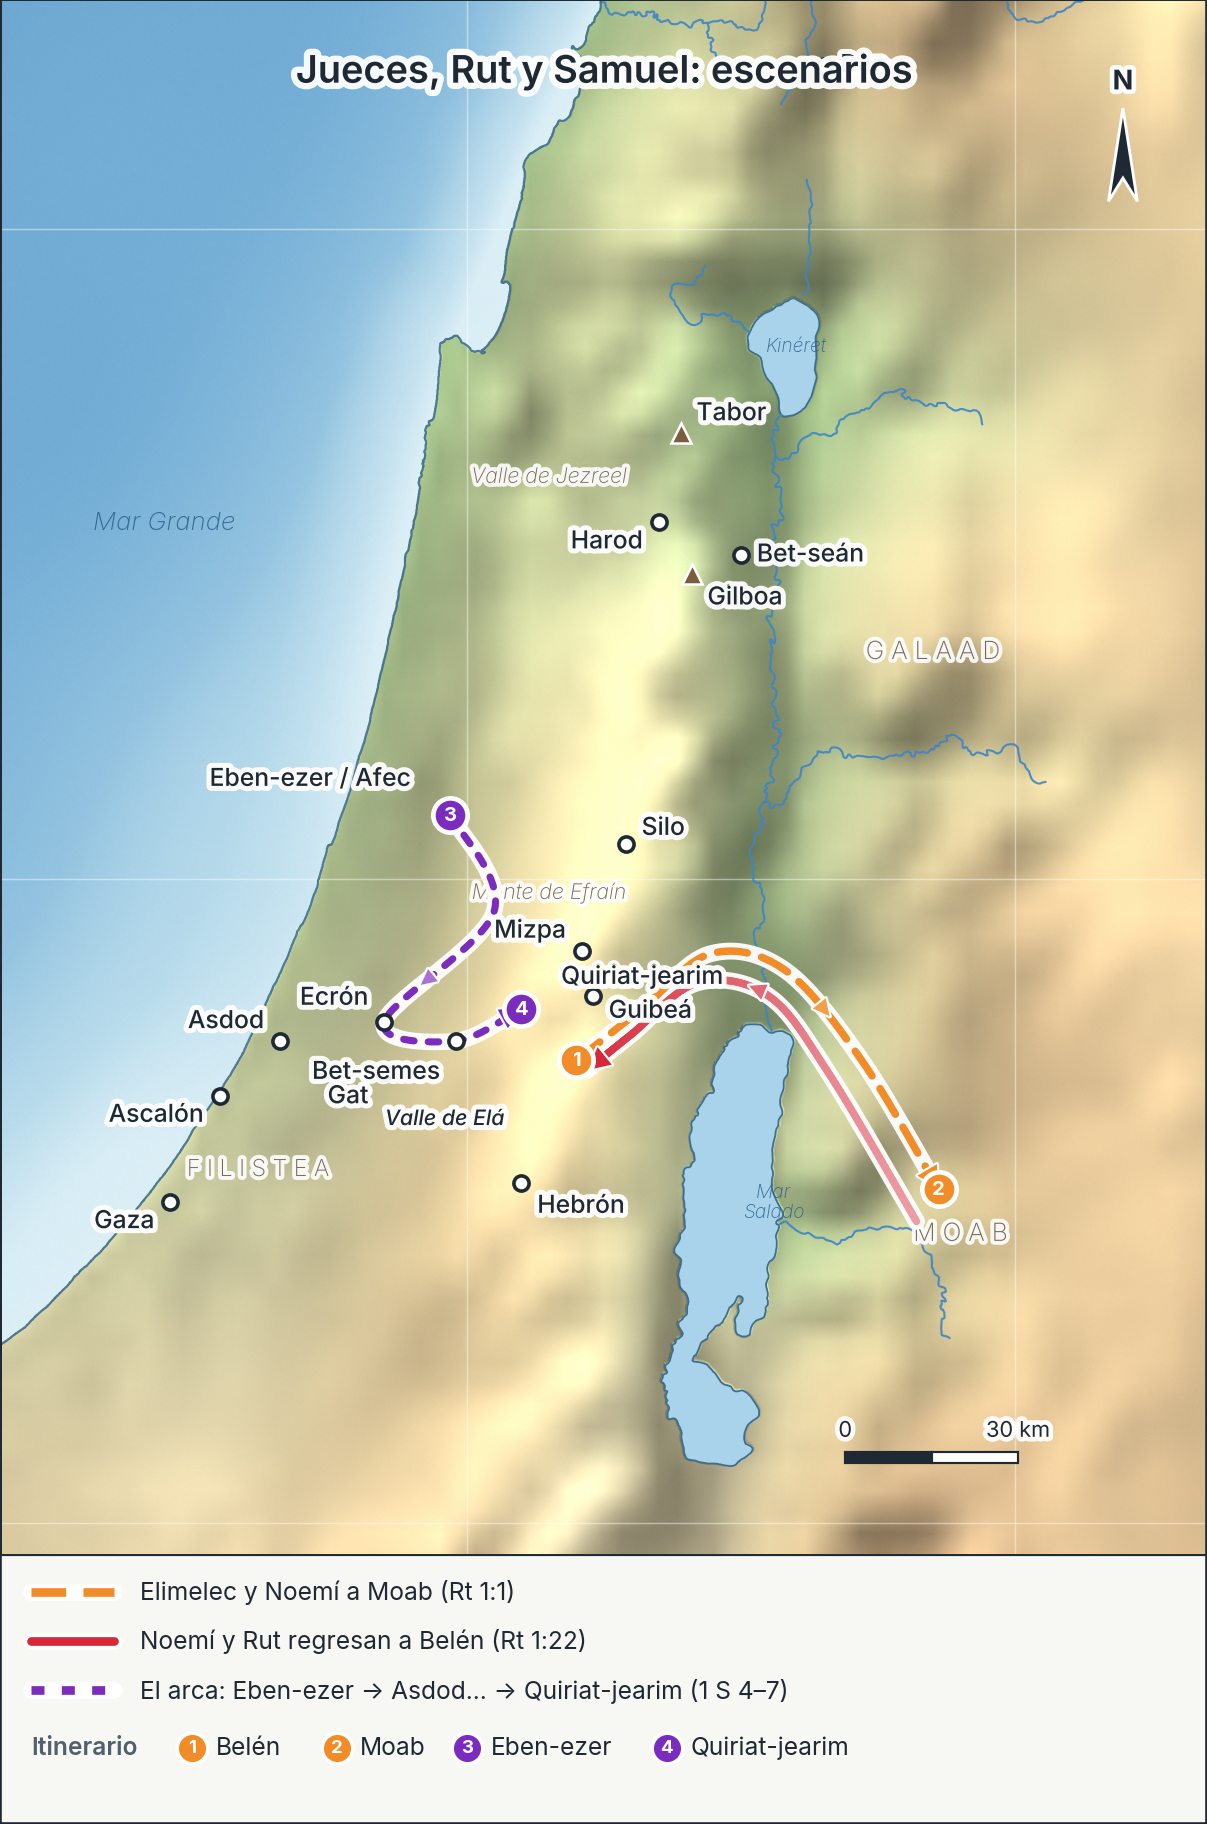
\includegraphics[width=0.42\linewidth]{mapa_jueces.png}\\[2pt]
{\footnotesize\color{sepia}\textit{Nota.} Elaboración propia: costas, lagos y ríos GSHHS/WDB y relieve sombreado (Basemap); ubicaciones antiguas aproximadas. }
\end{minipage}\end{center}

\subsection{Los filisteos}
El gran adversario de la segunda mitad del período son los filisteos, llegados con los «Pueblos del Mar»: los relieves de Medinet Habu muestran a Ramsés~III (c.~1177 a.\,e.\,c.) combatiendo a los \emph{Peleset}, el hebreo \heb{פְּלִשְׁתִּים} (\emph{pelishtím}). En Asdod, Ascalón, Ecrón y Gat aparece una cultura material de origen egeo, con cerámica monocroma y luego bícroma, hogares de tipo egeo y consumo de cerdo (Dothan, 1982).

La inscripción real de Ecrón, dedicada por «Akish, hijo de Padi, rey de Ecrón», muestra que Aquis, el rey de Gat de 1~S 21:10 [21:11] y 27:2, llevaba un nombre real filisteo, aunque es del siglo \textsc{vii} y no alude al personaje bíblico (Gitin et~al., 1997).

\subsection{Silo, Bet-semes y Khirbet Qeiyafa}
Silo, donde estaba el arca, tenía en el Hierro~I edificios con pilares y depósitos y fue destruida por un incendio hacia mediados del siglo \textsc{xi} a.\,e.\,c. (Finkelstein et~al., 1993). Muchos asocian esa destrucción con la derrota de Afec, y aunque Samuel no narra la caída de Silo, Jer 7:12--14 y Sal 78:60 la recuerdan; las excavaciones recientes del sitio siguen en proceso de publicación. Bet-semes, adonde vuelve el arca (1~S 6), era una población fronteriza con la llanura filistea, y sus excavadores ven en la escasez de cerdo una frontera cultural consciente frente a Ecrón (Bunimovitz y Lederman, 2009).

Sobre el valle de Ela, escenario del combate con Goliat, se levanta Khirbet Qeiyafa, fortaleza de unas 2,3 hectáreas con muralla de casamatas y dos puertas, fechada por radiocarbono hacia c.~1020--980 a.\,e.\,c. Sus excavadores la consideran una ciudad de Judá del tiempo de David y proponen identificarla con Saaraim, «las dos puertas» (1~S 17:52; Garfinkel et~al., 2016); Finkelstein y Fantalkin (2012) aceptan la fecha, pero la atribuyen a una entidad del norte, quizá la de Saúl, y otros la consideran cananea o filistea.

\section{Desarrollo bíblico}

\subsection{La espiral de los jueces y la ruina interior}
El prólogo de Jueces da la clave de lectura del libro antes de contar ninguna historia:

\begin{cita}Y los hijos de Israel hicieron lo malo ante los ojos de YHWH y sirvieron a los baales [\ldots]. Y YHWH levantó jueces que los libraron de mano de los que los saqueaban [\ldots], porque YHWH se compadecía de su gemido. Pero cuando moría el juez, volvían a corromperse más que sus padres.\fuente{(Jue 2:11, 16, 18--19)}\end{cita}

El esquema avanza de la apostasía a la opresión, del clamor (\heb{וַיִּזְעֲקוּ}, \emph{va-yiz'aqú}, Jue 3:9) al libertador y al reposo, pero cada vuelta deja al pueblo más abajo: la fórmula «y reposó la tierra» aparece tras Otoniel, Aod, Débora y Gedeón (3:11, 30; 5:31; 8:28) y después ya no vuelve, y las tribus terminan en guerra civil. El \heb{שֹׁפֵט} (\emph{shofet}) no es un magistrado de tribunal, sino un líder carismático que libra y gobierna, y el texto insiste en que YHWH lo «levanta», porque el verdadero juez es Él (Jue 11:27). Que Dios responda a un gemido y no a un arrepentimiento pleno es la semilla de la restauración posterior.

Los relatos muestran el descenso. Débora, «profetisa» que «juzgaba a Israel» (Jue 4:4), canta una victoria en que las tribus se miden por haber acudido o no «en ayuda de YHWH» (5:23). Gedeón vence a Madián con trescientos hombres «para que Israel no se alabe contra mí» (7:2) y, cuando se le ofrece una dinastía, la rechaza con la fórmula que mejor expresa el ideal teocrático del período: «No reinaré yo sobre vosotros, ni mi hijo reinará sobre vosotros; YHWH reinará sobre vosotros» (\heb{יְהוָה יִמְשֹׁל בָּכֶם}, Jue 8:23). Acto seguido fabrica un efod que «todo Israel prostituyó tras él» (8:27). La victoria sobre Madián, en cambio, quedará en la memoria profética como figura de la liberación futura (Is 9:4 [9:3]; 10:26). Con Jefté, cuyo voto trata a YHWH con la lógica de los dioses vecinos (11:30--40), los galaaditas degüellan a los efraimitas que dicen \heb{סִבֹּלֶת} (\emph{sibólet}) en lugar de \heb{שִׁבֹּלֶת} (\emph{shibólet}) (12:5--6), y con ello Israel empieza a matar a Israel.

Sansón, «nazareo de Dios desde el vientre» (\heb{נְזִיר אֱלֹהִים}, 13:5), nace como Isaac de una mujer estéril y recibe la misión de que «comenzará a salvar a Israel de mano de los filisteos», salvación que completarán Samuel y David (1~S 7:13; 2~S 8:1). Elige mujer porque «ella es recta a mis ojos» (14:3), anticipo del estribillo final del libro, y aun así Heb 11:32 lo cuenta entre los que actuaron «por la fe». En él se reconoce el Israel de la época, consagrado desde su origen, entregado a vivir como las naciones y nunca despojado de su llamado.

Los apéndices del libro descienden todavía más. Micaía contrata a un levita para su santuario de efod y terafines, convencido de que «YHWH me prosperará, porque tengo un levita por sacerdote» (17:13). La tribu de Dan se lleva ídolo y sacerdote y funda un santuario que dura «hasta el día del cautiverio de la tierra» (18:30), hilo que conduce al destierro asirio del reino del norte, pues en el mismo Dan pondrá Jeroboam uno de sus becerros (1~R 12:29).

\begin{nota}[Precisión textual: el nieto de Moisés (Jue 18:30)]
El sacerdote de Dan es «Jonatán, hijo de Gersón, hijo de \emph{Manasés}». En el TM la \emph{nun} de \heb{מנשה} está escrita suspendida sobre la línea; sin ella se lee \heb{משה}, «Moisés», cuyo hijo era Gersón (Éx 2:22). El Talmud explica que se añadió para no avergonzar a Moisés con la idolatría de su nieto (Bava Batra 109b), y varios manuscritos de la Septuaginta y la Vulgata leen «Moisés». De ser así, el primer sacerdote idólatra de Israel fue nieto del mediador del Sinaí.
\end{nota}

En Guibeá de Benjamín, por último, los hombres de la ciudad repiten casi palabra por palabra a los de Sodoma (19:22; cf. Gn 19:4--5); el levita había evitado Jebús «porque es ciudad de extranjeros» (19:12), y la ironía es deliberada. La guerra que sigue deja a Benjamín al borde de la extinción, y el pueblo llora: «¿Por qué, oh YHWH, Dios de Israel, ha sucedido esto, que falte hoy de Israel una tribu?» (21:3). Siglos más tarde Oseas hará de aquel episodio la medida de todos los pecados del reino del norte: «desde los días de Guibeá has pecado, oh Israel» (\heb{מִימֵי הַגִּבְעָה חָטָאתָ יִשְׂרָאֵל}, Os 10:9; cf. 9:9). El libro se cierra con su estribillo, «no había rey en Israel; cada uno hacía lo que era recto ante sus propios ojos» (\heb{אִישׁ הַיָּשָׁר בְּעֵינָיו יַעֲשֶׂה}, 21:25), eco de Dt 12:8. Es un estribillo de doble filo, porque prepara el terreno para la monarquía pero deja intacto el ideal de Gedeón: lo que falta en Israel no es tanto un monarca como alguien que busque lo recto a los ojos de Dios.

\subsection{Rut: la extranjera que se une a Israel}
Rut transcurre «en los días en que juzgaban los jueces» (Rt 1:1) y en la misma Belén, pero invierte el cuadro: donde Jueces muestra a israelitas que se comportan como cananeos, aquí una moabita se comporta como israelita fiel. Viuda, se niega a volver a Moab:

\hebverso{כִּי אֶל־אֲשֶׁר תֵּלְכִי אֵלֵךְ וּבַאֲשֶׁר תָּלִינִי אָלִין עַמֵּךְ עַמִּי וֵאלֹהַיִךְ אֱלֹהָי}
\begin{cita}Adonde tú vayas, iré yo; y donde tú pases la noche, la pasaré yo. Tu pueblo será mi pueblo, y tu Dios, mi Dios.\fuente{(Rt 1:16)}\end{cita}

Primero el pueblo y después Dios. Rut se une a Israel y, con él, a su Dios, como la promesa a Abraham lo anunciaba para «todas las familias de la tierra» (Gn 12:3); ese orden anticipa la imagen paulina de las ramas injertadas en el olivo. La palabra que da tono al libro es \heb{חֶסֶד} (\emph{jésed}), lealtad que va más allá de lo debido (1:8; 2:20; 3:10). Booz actúa como \heb{גֹּאֵל} (\emph{go'el}), el pariente redentor de Lv 25:25 que mantiene el nombre del difunto (cf. Dt 25:5--10), y las mujeres de Belén bendicen a Dios «que no te ha dejado hoy sin redentor» (4:14). La genealogía de diez generaciones, de Fares a David, termina con Obed, que «es el padre de Isaí, padre de David» (\heb{הוּא אֲבִי־יִשַׁי אֲבִי דָוִד}, 4:17), y convierte la historia familiar en prólogo de la monarquía y, para Mateo, del Mesías (Mt 1:5).

\subsection{Ana, Samuel y el anuncio del ungido}
1~Samuel empieza como empezó Israel, con una mujer estéril. Ana consagra a su hijo y entona un cántico de inversión de suertes, el del Dios que «levanta del polvo al pobre [\ldots] para hacerlo sentar con príncipes» (2:8), que termina con una palabra aplicada por primera vez a un rey:

\hebverso{יְהוָה יָדִין אַפְסֵי־אָרֶץ וְיִתֶּן־עֹז לְמַלְכּוֹ וְיָרֵם קֶרֶן מְשִׁיחוֹ}
\begin{cita}YHWH juzgará los confines de la tierra; dará poder a su rey y exaltará el poder de su ungido.\fuente{(1~S 2:10)}\end{cita}

Ana habla de «su rey» cuando Israel no tiene ninguno. La Septuaginta traduce \heb{מְשִׁיחוֹ} (\emph{meshijó}) por \grc{χριστοῦ αὐτοῦ}, y Zacarías retoma su «cuerno» al bendecir a Dios porque «nos levantó un cuerno de salvación en la casa de David» (\grc{ἤγειρεν κέρας σωτηρίας ἡμῖν ἐν οἴκῳ Δαυίδ}, Lc 1:69). Frente a Ana se alza la casa de Elí, cuyos hijos «no conocían a YHWH» (2:12), y el juicio sobre ella llega junto con una promesa: «me suscitaré un sacerdote fiel (\heb{כֹּהֵן נֶאֱמָן}) [\ldots]; le edificaré casa firme, y andará delante de mi ungido todos los días» (2:35). Dentro del relato, el sacerdote fiel es Samuel y, a más largo plazo, la línea de Sadoc (1~R 2:27, 35), y lo llamativo es que la promesa vuelva a hablar de un ungido. En días en que «la palabra de YHWH escaseaba» (3:1), Dios la renueva llamando de noche al niño Samuel, a quien todo Israel, «desde Dan hasta Beerseba», reconoce como profeta (3:20).

Tras la derrota de Afec, Israel trae el arca como un amuleto, «para que nos salve» (4:3); los filisteos la capturan, y la nuera de Elí llama a su hijo Icabod, «¿dónde está la gloria?»:

\hebverso{וַתִּקְרָא לַנַּעַר אִי־כָבוֹד לֵאמֹר גָּלָה כָבוֹד מִיִּשְׂרָאֵל}
\begin{cita}Y llamó al niño Icabod, diciendo: ¡Se ha ido la gloria de Israel!\fuente{(1~S 4:21)}\end{cita}

El verbo \heb{גָּלָה} (\emph{galá}) es el del destierro, y la gloria, en rigor, «ha ido al exilio». Pero el arca vuelve sola a Bet-semes (6:12), porque Dios no necesita a Israel para defender su gloria. Veinte años más tarde Samuel convoca al pueblo en Mizpa: «Si de todo vuestro corazón os volvéis a YHWH, quitad los dioses ajenos» (7:3). El pueblo ayuna y confiesa, Samuel intercede, Dios truena contra los filisteos, y en el mismo lugar de la derrota de 4:1 se levanta la piedra \heb{אֶבֶן הָעָזֶר} (\emph{Even ha-ézer}): «Hasta aquí nos ayudó YHWH» (\heb{עַד־הֵנָּה עֲזָרָנוּ יְהוָה}, 7:12). Mientras Israel trató el arca como un objeto, perdió; cuando volvió a Dios con arrepentimiento e intercesión, fue librado, y en 1~S 7 el ciclo de Jueces se cumple por fin como debía, bajo un juez que es a la vez profeta e intercesor. Exilio de la gloria, retorno y vuelta del corazón anticipan en pequeño el patrón que los profetas aplicarán a Babilonia.

\subsection{«Como todas las naciones» y el rechazo de Saúl}
Los hijos de Samuel «no anduvieron en sus caminos» (8:3), y los ancianos piden:

\hebverso{שִׂימָה־לָּנוּ מֶלֶךְ לְשָׁפְטֵנוּ כְּכָל־הַגּוֹיִם}
\begin{cita}Constitúyenos ahora un rey que nos juzgue, como tienen todas las naciones.\fuente{(1~S 8:5)}\end{cita}

Dios va al fondo: «no te han desechado a ti, sino a mí me han desechado, para que no reine sobre ellos» (8:7). La monarquía en sí misma no era el problema, porque la Torá la había previsto, «pondrás sobre ti por rey al que YHWH tu Dios escoja» (Dt 17:15), y la promesa a Abraham incluía reyes (Gn 17:6; cf. 49:10); pero el mismo pasaje le fija límites (Dt 17:14--20), y el rey no multiplicará caballos, mujeres ni oro y leerá la Torá todos los días. Lo que se discute es el modelo, y entre Éx 19:6 y 1~S 8:5 queda planteada la tensión entre ser «reino de sacerdotes» y ser «como todas las naciones».

Samuel unge a Saúl, un benjaminita, como \heb{נָגִיד} (\emph{naguid}), encargado de Dios sobre una heredad que sigue siendo de Dios (10:1). Su autoridad se confirma cuando libra a Jabes de Galaad (1~S 11), la ciudad arrasada en Jue 21, de modo que el rey benjaminita repara en cierto modo la historia de su propia tribu. En Gilgal, Samuel pronuncia la promesa que sostiene buena parte de esta serie:

\hebverso{כִּי לֹא־יִטֹּשׁ יְהוָה אֶת־עַמּוֹ בַּעֲבוּר שְׁמוֹ הַגָּדוֹל}
\begin{cita}Porque YHWH no desamparará a su pueblo, por causa de su gran nombre [\ldots]. Y en cuanto a mí, lejos sea de mí que peque contra YHWH dejando de rogar por vosotros.\fuente{(1~S 12:22--23)}\end{cita}

La permanencia descansa en el nombre de Dios y no en la fidelidad de un pueblo que acaba de rechazarlo. La Septuaginta traduce \grc{ὅτι οὐκ ἀπώσεται κύριος τὸν λαὸν αὐτοῦ}, y Pablo usará ese mismo verbo en Ro 11:1--2 (\grc{μὴ ἀπώσατο ὁ θεὸς τὸν λαὸν αὐτοῦ;}), con eco también de Sal 94:14 (93:14 en la LXX). Saúl, en cambio, ofrece él mismo el holocausto en Gilgal sin esperar a Samuel y oye que «YHWH se ha buscado un hombre conforme a su corazón» (\heb{בִּקֵּשׁ יְהוָה לוֹ אִישׁ כִּלְבָבוֹ}, 13:14); más tarde perdona a Agag y lo mejor del ganado de Amalec, y Samuel le responde que «obedecer es mejor que el sacrificio» (15:22). Como Micaía y como Israel en Afec, Saúl ha confundido el culto con un instrumento para conseguir resultados. El reino le es «rasgado» (15:27--28), con un lenguaje que volverá en la división del reino (1~R 11:30--31).

\begin{perla}{«no desechará a su pueblo»}
La frase con que Samuel funda la permanencia de Israel en el día en que el pueblo pide rey pasa, por medio de la Septuaginta, al centro de Romanos~11.\par\smallskip
{\centering\renewcommand{\arraystretch}{1.18}
\begin{tabular}{>{\RaggedRight\arraybackslash}p{2.2cm}>{\RaggedRight\arraybackslash}p{6.3cm}>{\RaggedRight\arraybackslash}p{5.5cm}}
\toprule
\textbf{Texto} & \textbf{Forma} & \textbf{Observación}\\
\midrule
1~S 12:22 TM & \heb{כִּי לֹא־יִטֹּשׁ יְהוָה אֶת־עַמּוֹ בַּעֲבוּר שְׁמוֹ הַגָּדוֹל} & La razón es el nombre de Dios y su voluntad de hacerlos «pueblo suyo»\\
1~S 12:22 LXX & \grc{ὅτι οὐκ ἀπώσεται κύριος τὸν λαὸν αὐτοῦ} & \emph{natash}, «abandonar», se vuelve \grc{ἀπωθέω}, «rechazar»\\
Sal 94:14 [93:14 LXX] & \grc{ὅτι οὐκ ἀπώσεται κύριος τὸν λαὸν αὐτοῦ} & La misma fórmula, ya convertida en confesión del salterio\\
Ro 11:1--2 & \grc{μὴ ἀπώσατο ὁ θεὸς τὸν λαὸν αὐτοῦ;} \ldots{} \grc{οὐκ ἀπώσατο} & Pablo convierte la promesa en pregunta y la responde con ella\\
\bottomrule
\end{tabular}\par}
\smallskip
La pregunta de Pablo no es retórica: usa el vocabulario de la promesa que cerró la época de los jueces, y su respuesta, «de ninguna manera», repite lo que Samuel dijo a un pueblo que acababa de rechazar a Dios como rey.
\end{perla}

\subsection{David, el menor, ungido en Belén}
En Belén, Dios corrige a Samuel ante Eliab, el primogénito de Isaí:

\hebverso{כִּי הָאָדָם יִרְאֶה לַעֵינַיִם וַיהוָה יִרְאֶה לַלֵּבָב}
\begin{cita}Porque el hombre mira lo que está delante de sus ojos, pero YHWH mira el corazón.\fuente{(1~S 16:7)}\end{cita}

El versículo contesta al estribillo de Jueces, porque a un pueblo que hacía «lo recto ante sus ojos» Dios le opone una elección basada en lo que ve en el corazón. Escoge al menor, el que estaba con las ovejas; «desde aquel día el Espíritu de YHWH vino sobre David» (16:13), al tiempo que se apartaba de Saúl (16:14), y el ungido de Ana tiene nombre. Frente a Goliat, que desafía a «los escuadrones del Dios viviente» (17:26), David declara que «toda la tierra sabrá que hay Dios en Israel» (\heb{וְיֵדְעוּ כָּל־הָאָרֶץ כִּי יֵשׁ אֱלֹהִים לְיִשְׂרָאֵל}, 17:46). La victoria persigue un fin misionero, y la vocación de Éx 19:6 reaparece en boca de un pastor de Belén.

Jonatán, heredero de Saúl, llega a decir a David: «tú reinarás sobre Israel, y yo seré segundo después de ti» (23:17). Saúl, en cambio, lo persigue movido por los celos y hace matar a los sacerdotes de Nob (22:18), con lo que se cumple sobre la casa de Elí la palabra de 2:31--33. David perdona dos veces la vida a Saúl, «el ungido de YHWH» (\heb{מְשִׁיחַ יְהוָה}, 24:6 [24:7]; 26:9--11), y Abigail le anuncia una «casa firme» (\heb{בַּיִת נֶאֱמָן}, 25:28), la expresión de 2:35 que anticipa 2~S 7.

Muerto Saúl, David es ungido sobre «la casa de Judá» en Hebrón (2~S 2:4), mientras Is-boset reina sobre «todo Israel» (2:9--10). Judá e Israel aparecen por primera vez como dos entidades políticas, aunque la distinción ya asomaba en 1~S 11:8 y 18:16 («todo Israel y Judá amaban a David»). David reunirá ambas casas en 2~S 5, y la división definitiva será tema del Estudio~4.

\section{Israel como nación santa y reino de sacerdotes}

El llamado de Éx 19:6 se resquebraja en estos siglos a la vista de todos. Israel adopta los dioses de Canaán en lugar de ser su luz (Jue 2:11--13; 3:5--6), con una idolatría cuya raíz está en el consejo de Balaam y el culto de Baal-peor (Nm 22--25; Ap 2:14). El sacerdocio se vende con el levita de Micaía, que se marcha con quien mejor le paga (Jue 18:19--20), y se corrompe en los hijos de Elí; el culto degenera en magia cuando el arca se lleva como amuleto o Saúl consulta a la adivina de Endor; y en Guibeá la ciudad israelita resulta más peligrosa que la extranjera Jebús. Balaam había dicho: «he aquí un pueblo que habitará solo, y no será contado entre las naciones» (Nm 23:9), y en 1~S 8:5, 20 es el propio pueblo el que pide ser contado entre ellas.

La vocación, sin embargo, no se extingue. Débora canta la victoria como obra de YHWH, y Rut lleva la bendición de Abraham a una mujer de las naciones conforme a la ley que preveía la incorporación del extranjero (Éx 12:48--49). Ana ora y profetiza, Jonatán reconoce la elección de Dios por encima de su derecho, y David combate para que la tierra conozca al Dios de Israel. Samuel, profeta y juez, ofrece sacrificios sin ser aaronita (1~S 7:9), pero ejerce sobre todo el oficio de intercesor (12:23), por el que Jeremías lo recordará junto a Moisés (Jer 15:1) y el salmista lo pondrá entre «los que invocaban su nombre» (Sal 99:6). En ellos continúa el remanente que comenzó con José (Gn 45:7), y Pablo lo dirá de su propio tiempo: «aun en este tiempo ha quedado un remanente escogido por gracia» (Ro 11:5).

\section{Aporte de la tradición judía}

La tradición rabínica, que debe distinguirse del texto bíblico, atribuye a Samuel la escritura de «su libro, Jueces y Rut» (Bava Batra 14b) y añade que, como 1~Samuel narra su muerte (1~S 25:1), lo completaron «Gad el vidente y Natán el profeta» (Bava Batra 15a; cf. 1~Cr 29:29); la crítica moderna sitúa la redacción final mucho después. Los rabinos contrastan a los dos primeros reyes: «Saúl falló en una cosa, y se le contó; David en dos, y no se le contó» (Yoma 22b), y el propio texto insinúa la razón, porque Saúl se justifica (1~S 15:20--21) y David confiesa (2~S 12:13).

Rut recibe una atención especial. La ley excluía al moabita de la congregación (Dt 23:3 [23:4]), pero la Mishná limita la prohibición a los varones (Yevamot 8:3) y el Talmud lo condensa en la frase «moabita, y no moabitesa» (Yevamot 76b--77a), con la que zanja la duda que Doeg el edomita plantea sobre la legitimidad de David; es una interpretación rabínica, no una distinción explícita de la Torá, y Esd 9--10 y Neh 13:1--3 aplican la ley de modo más estricto. Para el Midrash el libro existe por el \emph{jésed}: «Este rollo no contiene [leyes de] impureza ni de pureza [\ldots]. ¿Para qué fue escrito? Para enseñar cuán grande es la recompensa de los que practican la misericordia» (Rut Rabbah 2:14; Freedman y Simon, 1939). La sinagoga lee Rut en Shavuot porque la historia transcurre durante la siega, porque Rut acepta la Torá como Israel en el Sinaí y porque una tradición sostiene que David nació y murió en esa fiesta (Talmud de Jerusalén, Jagigá 2:3; Neusner, 1982--1994).

El cántico de Ana es la haftará del primer día de Rosh Hashaná junto con Gn 21, porque ambos textos dicen que Dios «visitó» a una estéril, \heb{וַיהוָה פָּקַד אֶת־שָׂרָה} (Gn 21:1) y \heb{כִּי־פָקַד יְהוָה אֶת־חַנָּה} (1~S 2:21), con el verbo \emph{paqad} que el Estudio~1 mostró como fórmula de redención. El Targum de Jonatán amplía ese mismo cántico en una profecía sobre la historia de Israel hasta los días del Mesías (Harrington y Saldarini, 1987). La haftará de la parashá Kóraj (1~S 11:14--12:22) presenta a Samuel defendiendo su integridad como Moisés ante Coré y termina precisamente con «YHWH no desamparará a su pueblo». La esperanza davídica sigue viva en la oración diaria, cuya decimoquinta bendición de la Amidá pide «haz brotar pronto el renuevo de David tu siervo» (\heb{אֶת־צֶמַח דָּוִד עַבְדְּךָ}), con el lenguaje de Jer 23:5, y la bendición después de las comidas pide misericordia «sobre el reino de la casa de David, tu ungido» (Sacks, 2009).

\section{La promesa de restauración}

Aun en el libro más sombrío, YHWH «se compadecía» (\heb{יִנָּחֵם}, \emph{yinnajem}) del gemido de su pueblo (Jue 2:18), hasta que «su alma no pudo soportar más la aflicción de Israel» (10:16). Sobre esa compasión sin mérito los textos de la etapa forman una cadena que los profetas retomarán.

\begin{center}\small
\renewcommand{\arraystretch}{1.25}
\begin{tabular}{>{\RaggedRight\arraybackslash}p{2.6cm}>{\RaggedRight\arraybackslash}p{5.0cm}>{\RaggedRight\arraybackslash}p{6.3cm}}
\toprule
\textbf{Texto} & \textbf{Promesa} & \textbf{Proyección}\\
\midrule
Jue 2:16, 18 & Dios levanta libertadores por compasión & Is 1:26 (jueces como al principio)\\
Jue 7--8 & La victoria sobre Madián & Is 9:4 [9:3]; 10:26 («como el día de Madián»)\\
Rt 4:14--17 & Un redentor (\emph{go'el}) y el linaje de David & Is 59:20; Ro 11:26 («vendrá de Sion el Libertador»)\\
1~S 2:10 & YHWH exaltará el poder de su ungido & Sal 2:2; Lc 1:69\\
1~S 2:35 & Un sacerdote fiel y una casa firme & 1~S 25:28; 2~S 7:16 (Estudio~4)\\
1~S 12:22 & YHWH no desamparará a su pueblo & Sal 94:14; Ro 11:1--2\\
1~S 13:14; 16:7 & Un hombre según el corazón de Dios & Jer 3:15; Hch 13:22\\
1~S 16:1, 13 & El ungido de Belén, hijo de Isaí & Is 11:1, 10; Mi 5:2 [5:1]; Ro 15:12\\
1~S 17:46 & «Toda la tierra sabrá que hay Dios en Israel» & Is 55:3--5 (David, testigo a los pueblos)\\
\bottomrule
\end{tabular}\end{center}

\subsection{Isaías: jueces restaurados y el renuevo de Isaí}
Isaías, ante una Jerusalén corrompida, anuncia el retorno al ideal de los jueces que Dios levantaba:

\hebverso{וְאָשִׁיבָה שֹׁפְטַיִךְ כְּבָרִאשֹׁנָה וְיֹעֲצַיִךְ כְּבַתְּחִלָּה}
\begin{cita}Restauraré tus jueces como al principio, y tus consejeros como al comienzo; entonces te llamarán Ciudad de justicia, Ciudad fiel.\fuente{(Is 1:26)}\end{cita}

El verbo \heb{וְאָשִׁיבָה} (\emph{ve-ashívah}) procede de \emph{shuv}, la raíz del regreso, y hace de aquella época un modelo de lo que Dios restaurará. La liberación del yugo asirio será «como en el día de Madián» (\heb{כְּיוֹם מִדְיָן}, Is 9:4 [9:3]) y «como la matanza de Madián en la peña de Oreb» (10:26; cf. Jue 7:25), y en el mismo oráculo nace el niño que reinará «sobre el trono de David» (9:7 [9:6]), de modo que la victoria de los trescientos pasa a ser figura de la salvación que traerá el rey davídico. Cuando la casa de David parezca un tronco talado, brotará algo nuevo de la familia de Belén:

\hebverso{וְיָצָא חֹטֶר מִגֵּזַע יִשָׁי וְנֵצֶר מִשָּׁרָשָׁיו יִפְרֶה}
\begin{cita}Saldrá una vara del tronco de Isaí, y un vástago brotará de sus raíces. Y reposará sobre él el Espíritu de YHWH.\fuente{(Is 11:1--2)}\end{cita}

Isaías no dice «tronco de David», sino «de Isaí», y vuelve al origen humilde de 1~S 16; el Espíritu que vino sobre David reposará sobre el vástago, y la raíz de Isaí será «estandarte a los pueblos» que las naciones buscarán (Is 11:10, citado en Ro 15:12). Is 32:1 anuncia que «para justicia reinará un rey». Las «misericordias firmes de David» (\heb{חַסְדֵי דָוִד הַנֶּאֱמָנִים}, Is 55:3) reúnen el \emph{jésed} de Rut y la «casa firme» de 1~S 2:35, y el oráculo añade «lo di por testigo a los pueblos» (55:4), con lo que en la figura del rey se concentra la misión de Israel hacia las naciones que David proclamó frente a Goliat.

\subsection{Jeremías: Silo, el Renuevo justo y «David su rey»}
Jeremías recurre a esta etapa, en primer lugar, como advertencia: «Andad ahora a mi lugar en Silo [\ldots] y ved lo que le hice por la maldad de mi pueblo Israel» (Jer 7:12; cf. 26:6). La pérdida de Silo y del arca prefigura la destrucción del Primer Templo (Estudio~5). Pero el profeta encuentra en ella también motivo de esperanza: retomando 1~S 13:14, Dios promete «pastores según mi corazón» (\heb{רֹעִים כְּלִבִּי}, Jer 3:15) y anuncia al rey que vendrá:

\hebverso{הִנֵּה יָמִים בָּאִים נְאֻם־יְהוָה וַהֲקִמֹתִי לְדָוִד צֶמַח צַדִּיק}
\begin{cita}He aquí que vienen días, dice YHWH, en que levantaré a David un Renuevo justo, y reinará como Rey [\ldots]. En sus días será salvo Judá, e Israel habitará confiado; y este será su nombre: YHWH, justicia nuestra.\fuente{(Jer 23:5--6; cf. 33:15--16)}\end{cita}

El oráculo nombra por separado a Judá, el reino del sur, y a Israel, aquí el reino del norte, ya desterrado por Asiria cuando habla Jeremías. El rey davídico salvará a ambos, y asoma así la reunificación que el Estudio~5 desarrollará a partir de Ez 37. Jer 30:9 lo condensa en una línea: «servirán a YHWH su Dios y a David su rey, a quien yo les levantaré».

\subsection{Oseas y Miqueas}
Oseas, profeta del reino del norte (aquí «Israel» designa ese reino), enlaza el comienzo y el final de esta etapa. Denuncia el pecado que viene «desde los días de Guibeá» (Os 9:9; 10:9) y el rey dado «en mi furor» (13:11), en alusión a 1~S 8, y aun así anuncia el regreso:

\hebverso{אַחַר יָשֻׁבוּ בְּנֵי יִשְׂרָאֵל וּבִקְשׁוּ אֶת־יְהוָה אֱלֹהֵיהֶם וְאֵת דָּוִד מַלְכָּם}
\begin{cita}Porque muchos días estarán los hijos de Israel sin rey, sin príncipe, sin sacrificio, sin estatua, sin efod y sin terafines. Después volverán los hijos de Israel y buscarán a YHWH su Dios y a David su rey.\fuente{(Os 3:4--5)}\end{cita}

La lista evoca el efod de Gedeón (Jue 8:27) y los terafines de Micaía (Jue 17:5), el verbo vuelve a ser \emph{shuv}, y la promesa es que el reino del norte, separado de la casa de David, regresará a «David su rey». ONE FOR ISRAEL (2025) cuenta este texto entre los que anuncian un regreso futuro del pueblo judío a Dios por medio del Mesías. Miqueas, por su parte, vuelve la mirada a la pequeña ciudad de Rut, Isaí y David: «Pero tú, Belén Efrata, pequeña para estar entre las familias de Judá, de ti me saldrá el que será gobernante en Israel» (\heb{מִמְּךָ לִי יֵצֵא לִהְיוֹת מוֹשֵׁל בְּיִשְׂרָאֵל}, Mi 5:2 [5:1]). «Efrata» es el clan de Elimelec (Rt 1:2) y de Isaí (1~S 17:12), y Mt 2:6 aplica el texto al nacimiento de Jesús.

\subsection{La lectura de Pablo}
Pablo recoge estos hilos. En Antioquía de Pisidia resume los jueces «hasta el profeta Samuel», el pedido de rey, a Saúl «de la tribu de Benjamín» y a David, combinando 1~S 13:14 y Sal 89:20 [89:21]: \grc{εὗρον Δαυὶδ τὸν τοῦ Ἰεσσαί, ἄνδρα κατὰ τὴν καρδίαν μου}, «he hallado a David, hijo de Isaí, varón conforme a mi corazón» (Hch 13:22), de cuya descendencia, «conforme a la promesa, Dios trajo a Israel un Salvador, Jesús» (13:23). La carta que culmina en Romanos 11 se abre con el Hijo «que nació del linaje de David según la carne» (\grc{τοῦ γενομένου ἐκ σπέρματος Δαυὶδ κατὰ σάρκα}, Ro 1:3). En el capítulo 11 la pregunta decisiva recibe la respuesta de 1~S 12:22: «¿Ha desechado Dios a su pueblo? En ninguna manera. Porque también yo soy israelita, de la descendencia de Abraham, de la tribu de Benjamín» (11:1); «No ha desechado Dios a su pueblo, al cual antes conoció» (\grc{οὐκ ἀπώσατο ὁ θεὸς τὸν λαὸν αὐτοῦ}, 11:2). Evoca luego a Elías y a los siete mil, y concluye que «aun en este tiempo ha quedado un remanente escogido por gracia» (11:5).

Lo afirma un benjaminita, de la tribu que casi desapareció en Jue 21 y de la que salió Saúl, el rey rechazado, cuyo nombre hebreo lleva el propio Pablo (Hch 13:9; Flp 3:5). Que sea precisamente él quien pregunte si Dios desechó a su pueblo y se presente como prueba de lo contrario tiene un peso particular, coincidencia que señala este estudio y no el apóstol. Ro 11:26 cita además Is 59:20, «vendrá de Sion el Libertador», donde el hebreo dice \heb{גּוֹאֵל} (\emph{go'el}), el título de Booz; Pablo sigue una forma cercana a la Septuaginta, «desde Sion» (\grc{ἐκ Σιών}), donde el TM lee «a Sion» (Moo, 1996). La conexión con Booz la propone este estudio, y el análisis del versículo corresponde al Estudio~8.

\section{Conclusión y puente al Estudio 4}

Entre los jueces y David, Israel pierde su vocación desde dentro, por la idolatría, por un sacerdocio comprado y por el deseo de parecerse a las naciones. En esa misma ruina la promesa de restauración toma forma: Dios se compadece de un gemido, guarda un remanente en el que figuran varias mujeres y una extranjera, anuncia con Ana un ungido que recibirá nombre en Belén y jura por boca de Samuel que no desamparará a su pueblo por causa de su nombre. Isaías hará de esa memoria la promesa de jueces restaurados y de un vástago de Isaí; Jeremías, la de un Renuevo que salvará a Judá y a Israel; Oseas, la del regreso del norte a «David su rey». Cuando Pablo, benjaminita, niega que Dios haya desechado a Israel, no improvisa un consuelo, porque repite lo que Samuel dijo a un pueblo que acababa de rechazar a Dios como rey.

Al terminar la etapa hay un rey ungido, pero el reino sigue incompleto: David reina en Hebrón sobre Judá, mientras la casa de Saúl conserva el resto de Israel (2~S 2:4, 9--10). El Estudio~4, \emph{de David a la división del reino}, seguirá a David hasta Jerusalén, el regreso del arca y la promesa de una casa eterna (2~S 7), y luego a Salomón, el templo y las causas de la división entre Israel (reino del norte) y Judá (reino del sur).

\section*{Preguntas para la reflexión}\markboth{Preguntas para la reflexión}{}
\begin{enumerate}
\item Israel pidió un rey «como todas las naciones» (1~S 8:5). ¿Bajo qué formas aparece hoy el deseo de que el pueblo de Dios se asemeje a su entorno?
\item Rut dijo «tu pueblo será mi pueblo, y tu Dios mi Dios» (Rt 1:16). ¿Qué enseña su orden a los creyentes de las naciones sobre su relación con Israel (Ro 11:17--18)?
\item «Obedecer es mejor que el sacrificio» (1~S 15:22). ¿Cómo distinguir el culto como obediencia del culto como medio para obtener resultados, como en Afec o en el santuario de Micaía?
\item ¿Qué relación hay entre la promesa de 1~S 12:22, la preservación de Benjamín en Jue 21 y el remanente de Ro 11:1--5?
\end{enumerate}

\section*{Glosario}\markboth{Glosario}{}
\begin{description}\small
\item[Eben-ezer] (\heb{אֶבֶן הָעָזֶר}). «Piedra de la ayuda». Memorial de Samuel tras la victoria de Mizpa (1~S 7:12).
\item[Go'el] (\heb{גֹּאֵל}). Pariente redentor que rescata la tierra o la persona de un familiar (Lv 25:25; Rt 4:14). Título de Dios en Isaías (Is 59:20).
\item[Icabod] (\heb{אִי־כָבוֹד}). «¿Dónde está la gloria?». Nombre del nieto de Elí al ser capturada el arca (1~S 4:21).
\item[Jésed] (\heb{חֶסֶד}). Lealtad amorosa, misericordia fiel; palabra clave de Rut (Rt 1:8; 2:20; 3:10).
\item[Kejol ha-goyim] (\heb{כְּכָל־הַגּוֹיִם}). «Como todas las naciones». Fórmula del pedido de rey (1~S 8:5, 20; cf. Dt 17:14).
\item[Mashíaj] (\heb{מָשִׁיחַ}; gr. \grc{χριστός}). Ungido. Aplicado al rey en 1~S 2:10; 16:6; 24:6 [24:7].
\item[Naguid] (\heb{נָגִיד}). Príncipe o designado; título de Saúl y de David como encargados de Dios (1~S 10:1; 13:14).
\item[Shofet] (\heb{שֹׁפֵט}). Juez; líder levantado por Dios para librar y gobernar al pueblo (Jue 2:16).
\item[Tsémaj] (\heb{צֶמַח}). Renuevo, brote; título del rey davídico futuro (Jer 23:5; 33:15).
\item[Yashar be-einav] (\heb{הַיָּשָׁר בְּעֵינָיו}). «Lo recto ante sus ojos». Estribillo de Jueces (17:6; 21:25), frente a lo recto ante los ojos de YHWH (Dt 12:8, 25).
\end{description}

\section*{Referencias}\markboth{Referencias}{}
\refapa{\emph{Biblia Hebraica Stuttgartensia} (5.ª ed.). (1997). Deutsche Bibelgesellschaft.}
\refapa{Bunimovitz, S., \& Lederman, Z. (2009). The archaeology of border communities: Renewed excavations at Tel Beth-Shemesh, Part 1: The Iron Age. \emph{Near Eastern Archaeology, 72}(3), 114--142.}
\refapa{Danby, H. (Trad.). (1933). \emph{The Mishnah}. Oxford University Press.}
\refapa{Dothan, T. (1982). \emph{The Philistines and their material culture}. Yale University Press.}
\refapa{Epstein, I. (Ed.). (1935--1948). \emph{The Babylonian Talmud}. Soncino Press.}
\refapa{Faust, A. (2006). \emph{Israel's ethnogenesis: Settlement, interaction, expansion and resistance}. Equinox.}
\refapa{Finkelstein, I. (1988). \emph{The archaeology of the Israelite settlement}. Israel Exploration Society.}
\refapa{Finkelstein, I., Bunimovitz, S., \& Lederman, Z. (1993). \emph{Shiloh: The archaeology of a biblical site}. Institute of Archaeology, Tel Aviv University.}
\refapa{Finkelstein, I., \& Fantalkin, A. (2012). Khirbet Qeiyafa: An unsensational archaeological and historical interpretation. \emph{Tel Aviv, 39}(1), 38--63.}
\refapa{Freedman, H., \& Simon, M. (Eds.). (1939). \emph{Midrash Rabbah}. Soncino Press.}
\refapa{Garfinkel, Y., Kreimerman, I., \& Zilberg, P. (2016). \emph{Debating Khirbet Qeiyafa: A fortified city in Judah from the time of King David}. Israel Exploration Society.}
\refapa{Gitin, S., Dothan, T., \& Naveh, J. (1997). A royal dedicatory inscription from Ekron. \emph{Israel Exploration Journal, 47}(1--2), 1--16.}
\refapa{Guggenheimer, H.~W. (1998). \emph{Seder Olam: The rabbinic view of biblical chronology}. Jason Aronson.}
\refapa{Harrington, D.~J., \& Saldarini, A.~J. (1987). \emph{Targum Jonathan of the Former Prophets} (The Aramaic Bible, Vol. 10). Michael Glazier.}
\refapa{Hesse, B., \& Wapnish, P. (1997). Can pig remains be used for ethnic diagnosis in the ancient Near East? En N.~A. Silberman \& D.~B. Small (Eds.), \emph{The archaeology of Israel: Constructing the past, interpreting the present}. Sheffield Academic Press.}
\refapa{Moo, D.~J. (1996). \emph{The epistle to the Romans}. Eerdmans.}
\refapa{Neusner, J. (Trad.). (1982--1994). \emph{The Talmud of the Land of Israel}. University of Chicago Press.}
\refapa{\emph{Novum Testamentum Graece} (28.ª ed.). (2012). Deutsche Bibelgesellschaft.}
\refapa{ONE FOR ISRAEL Ministry. (2025, 3 de julio). \emph{What does «all Israel will be saved» mean in Romans 11?} \url{https://www.oneforisrael.org/what-does-all-israel-will-be-saved-mean-in-romans-11/}}
\refapa{Rahlfs, A., \& Hanhart, R. (Eds.). (2006). \emph{Septuaginta} (ed. rev.). Deutsche Bibelgesellschaft.}
\refapa{Sacks, J. (Trad.). (2009). \emph{The Koren Siddur}. Koren Publishers.}
\refapa{Stager, L.~E. (1985). The archaeology of the family in ancient Israel. \emph{Bulletin of the American Schools of Oriental Research, 260}, 1--35.}
\end{document}
